\documentclass[10pt,letterpaper]{article}
\usepackage[margin=.65in]{geometry}
\usepackage{amsmath,graphicx,xcolor,feynman-fun}
\setlength{\parindent}{0pt}
\definecolor{tracez}{RGB}{30,80,150}
\newcommand{\heading}[2]{{\sffamily\bfseries\Large #1}\par\medskip #2\par\bigskip}
% Source traces are specifications, not public recipes for unsupported routing.
\newcommand{\tracediagram}[1]{%
 \begin{tikzpicture}[scale=.8,baseline=(current bounding box.center)]
  \coordinate(q1)at(-2.1,2.1);\coordinate(q2)at(-2.1,-2.1);
  \coordinate(q3)at(2.1,2.1);\coordinate(q4)at(2.1,-2.1);
  \ifnum#1=14
   \coordinate(Q)at(0,1.1);\coordinate(A)at(-1.1,-1.1);\coordinate(B)at(1.1,-1.1);
   \draw(q1)--(Q);\draw(q2)--(A);\draw(q3)--(B);
   \coordinate(X)at(intersection of Q--q4 and B--q3);
   \draw(Q)--($(X)!4pt!(Q)$);\draw($(X)!4pt!(q4)$)--(q4);
   \draw(Q)--(A);\draw(Q)--(B);
   \node[above=3pt]at(Q){$Q$};\node[left=3pt]at(A){$A$};\node[below=4pt]at(B){$B$};
  \else
   \coordinate(Q)at(0,-1.1);\coordinate(A)at(-1.1,1.1);\coordinate(B)at(1.1,1.1);
   \draw(q1)--(A);\draw(q2)--(Q);\draw(q4)--(B);
   \coordinate(X)at(intersection of Q--q3 and B--q4);
   \draw(Q)--($(X)!4pt!(Q)$);\draw($(X)!4pt!(q3)$)--(q3);
   \draw(A)--(Q);\draw(B)--(Q);
   \node[below=3pt]at(Q){$Q$};\node[left=3pt]at(A){$A$};\node[above=4pt]at(B){$B$};
  \fi
  \draw[tracez,line width=.8pt](A)--node[above]{$Z$}(B);
  \foreach\v in{Q,A,B}{\filldraw[black](\v)circle[radius=2.15pt];}
  \node[above left]at(q1){$q_1$};\node[below left]at(q2){$q_2$};
  \node[above right]at(q3){$q_3$};\node[below right]at(q4){$q_4$};
 \end{tikzpicture}}
\newcommand{\existing}[2]{\begin{minipage}[t][2.77in][t]{.48\linewidth}
 \textbf{#1}\par\medskip\centering
 \TriangleContactCorr[field={},central={},show-momenta=false,
  leg-labels={q_1,q_2,q_3,q_4},triangle-contact-line=plain,
  triangle-contact-external-line=plain,triangle-contact-internal-line=plain,
  triangle-contact-xspan=1.1,triangle-contact-yspan=1.1,
  triangle-contact-orientation=#2]
 \par\medskip\raggedright{\ttfamily\small triangle-contact-orientation=#2}
 \end{minipage}}
\newcommand{\styled}[2]{\TriangleContactCorr[field={},central={},show-momenta=false,
 leg-labels={q_1,q_2,q_3,q_4},triangle-contact-orientation=#1,
 triangle-contact-xspan=1.1,triangle-contact-yspan=1.1,
 triangle-contact-external-line=ewboson,triangle-contact-internal-lines={#2}]}
\begin{document}
\heading{M07c: trace the original connections}{S13-left/right from the supplied PowerPoint. External numbers use the established positions: 1 UL, 2 LL, 3 UR, 4 LR. The right-side crossover has no interaction dot.}
\textbf{S13-left: quartic pair 1/4; Z joins the q2/q3 vertices}\par\medskip
\begin{minipage}{.49\linewidth}\centering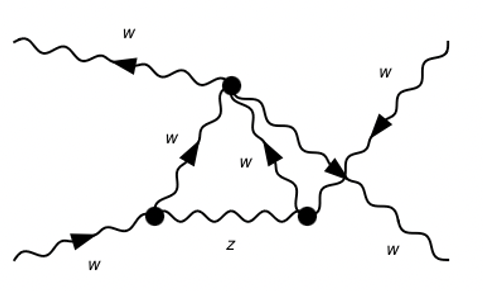
\includegraphics[width=.97\linewidth]{source-panels/S13-left.png}\par\small Original native image\end{minipage}\hfill
\begin{minipage}{.48\linewidth}\centering\tracediagram{14}\par\small Connectivity trace (target; routing not implemented)\end{minipage}
\par\medskip $Q$ is quartic; $A,B$ are trivalent. Slots: $1\to Q$, $2\to A$, $3\to B$, $4\to Q$. Internal edges: $Q$--$A$ (W), $Q$--$B$ (W), $A$--$B$ (Z).
\par\vspace{18pt}
\textbf{S13-right: quartic pair 2/3; Z joins the q1/q4 vertices}\par\medskip
\begin{minipage}{.49\linewidth}\centering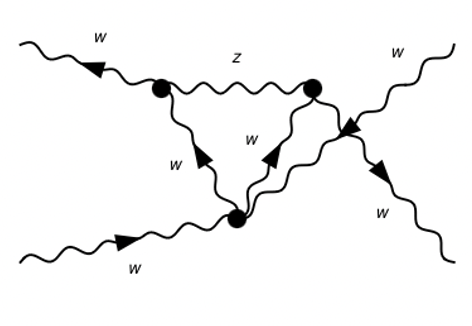
\includegraphics[width=.97\linewidth]{source-panels/S13-right.png}\par\small Original native image\end{minipage}\hfill
\begin{minipage}{.48\linewidth}\centering\tracediagram{23}\par\small Connectivity trace (target; routing not implemented)\end{minipage}
\par\medskip Slots: $1\to A$, $2\to Q$, $3\to Q$, $4\to B$. Internal edges are the same W/W/Z triangle. Each panel has 7 logical edges, 3 interaction vertices, valences 4/3/3 and one loop.
\newpage
\heading{Current public triangle-contact recipes}{These four outputs use the existing public package. They cover adjacent quartic pairs. The sources require opposite pairs 1/4 and 2/3, with fixed outer endpoints.}
\existing{Top: quartic pair 1/3}{top}\hfill\existing{Bottom: quartic pair 2/4}{bottom}\par
\existing{Left: quartic pair 1/2}{left}\hfill\existing{Right: quartic pair 3/4}{right}
Equal 1.1 internal half-spans demonstrate an existing square bounding-frame option. Changing spans or external label text does not supply the missing fixed-slot attachments. The target is a triangle contact with crossed external routing, with three interaction vertices.
\newpage
\heading{Existing styling and the missing routing slice}{R14's diagonal external-pair wording is consistent with S13 under fixed spatial numbering. The internal Z connects interaction vertices carrying those single external legs. This correspondence is an inference from the two references.}
\textbf{Existing recipes below support the loop and Z styling; external routing differs}\par\medskip
\begin{minipage}{.48\linewidth}\centering\styled{top}{ewboson,{ewboson,circ=Z},ewboson}\par\small Top orientation: Z is internal slot 6. Current quartic pair 1/3; source requires 1/4.\end{minipage}\hfill
\begin{minipage}{.48\linewidth}\centering\styled{bottom}{{ewboson,circ=Z},ewboson,ewboson}\par\small Bottom orientation: Z is internal slot 5. Current quartic pair 2/4; source requires 2/3.\end{minipage}
\par\bigskip\textbf{Precise missing slice}\par\medskip
Reuse TriangleContactCorr and its seven logical propagator slots. For the top source, keep slot 1 at Q and slot 2 at A, move slot 3 to B and slot 4 to Q. For the bottom source, keep slot 1 at A and slot 2 at Q, move slot 3 to Q and slot 4 to B. Keep outer endpoints fixed. The quartic-to-right external leg needs a crossing gap, with no new vertex or marker at its cut.
\par\medskip
Styles, circles, caps, momenta and indices must follow logical slots. Preserve all four current orientations. Square internal bounding spans already have public controls; exact visual tuning remains a future coding-session choice.
\par\bigskip\textbf{Audit conclusion}\par\medskip
R14 and R22 identify the same missing external-routing extension of an existing loop family. The trace resolves the source question; it does not implement that extension. The ordinary-box right external crossing (R04) remains separately deferred by the user.
\par\medskip
Package code is unchanged. The next scheduled coding session is M08a contact-leg bubbles. The triangle-contact routing follow-up remains unscheduled unless requested.
\end{document}
